\chapter{Resultados complementarios do procesamento automático}
\label{app:resultados-procesamento}

\section{Adestramento do modelo personalizado de Tesseract}

A Figura~\ref{fig:anexo-bcer-tesseract} mostra a evolución do \gls{bcer}
durante o adestramento do modelo \textit{sintromv2}. A taxa de erro diminuíu
progresivamente ata alcanzar o seu mellor resultado na iteración 4\,911.

\begin{figure}[htbp]
    \centering
    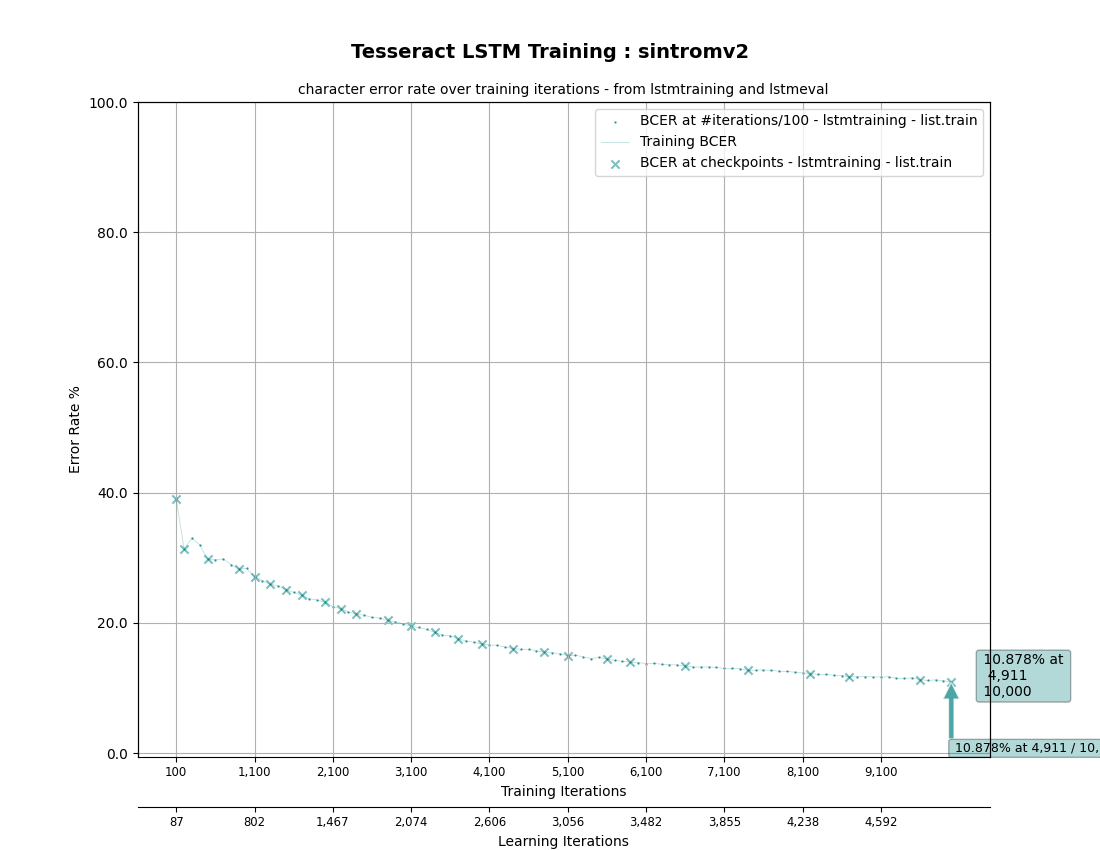
\includegraphics[width=0.92\textwidth]{imaxes/06-Procesamento automático das follas de tratamento/sintromv2.plot_cer.png}
    \caption{Evolución do BCER durante o adestramento do modelo
    \textit{sintromv2}.}
    \label{fig:anexo-bcer-tesseract}
\end{figure}

\FloatBarrier

\section{Avaliación do detector YOLO}

As Figuras~\ref{fig:anexo-yolo-pr} e~\ref{fig:anexo-yolo-confusion}
representan os resultados completos obtidos durante a validación do detector.
A curva Precision-Recall permite observar a relación entre a precisión e a
capacidade do modelo para localizar as representacións das pastillas. Pola
súa parte, a matriz de confusión recolle as deteccións correctas, os falsos
positivos e os elementos non detectados.

\begin{figure}[htbp]
    \centering
    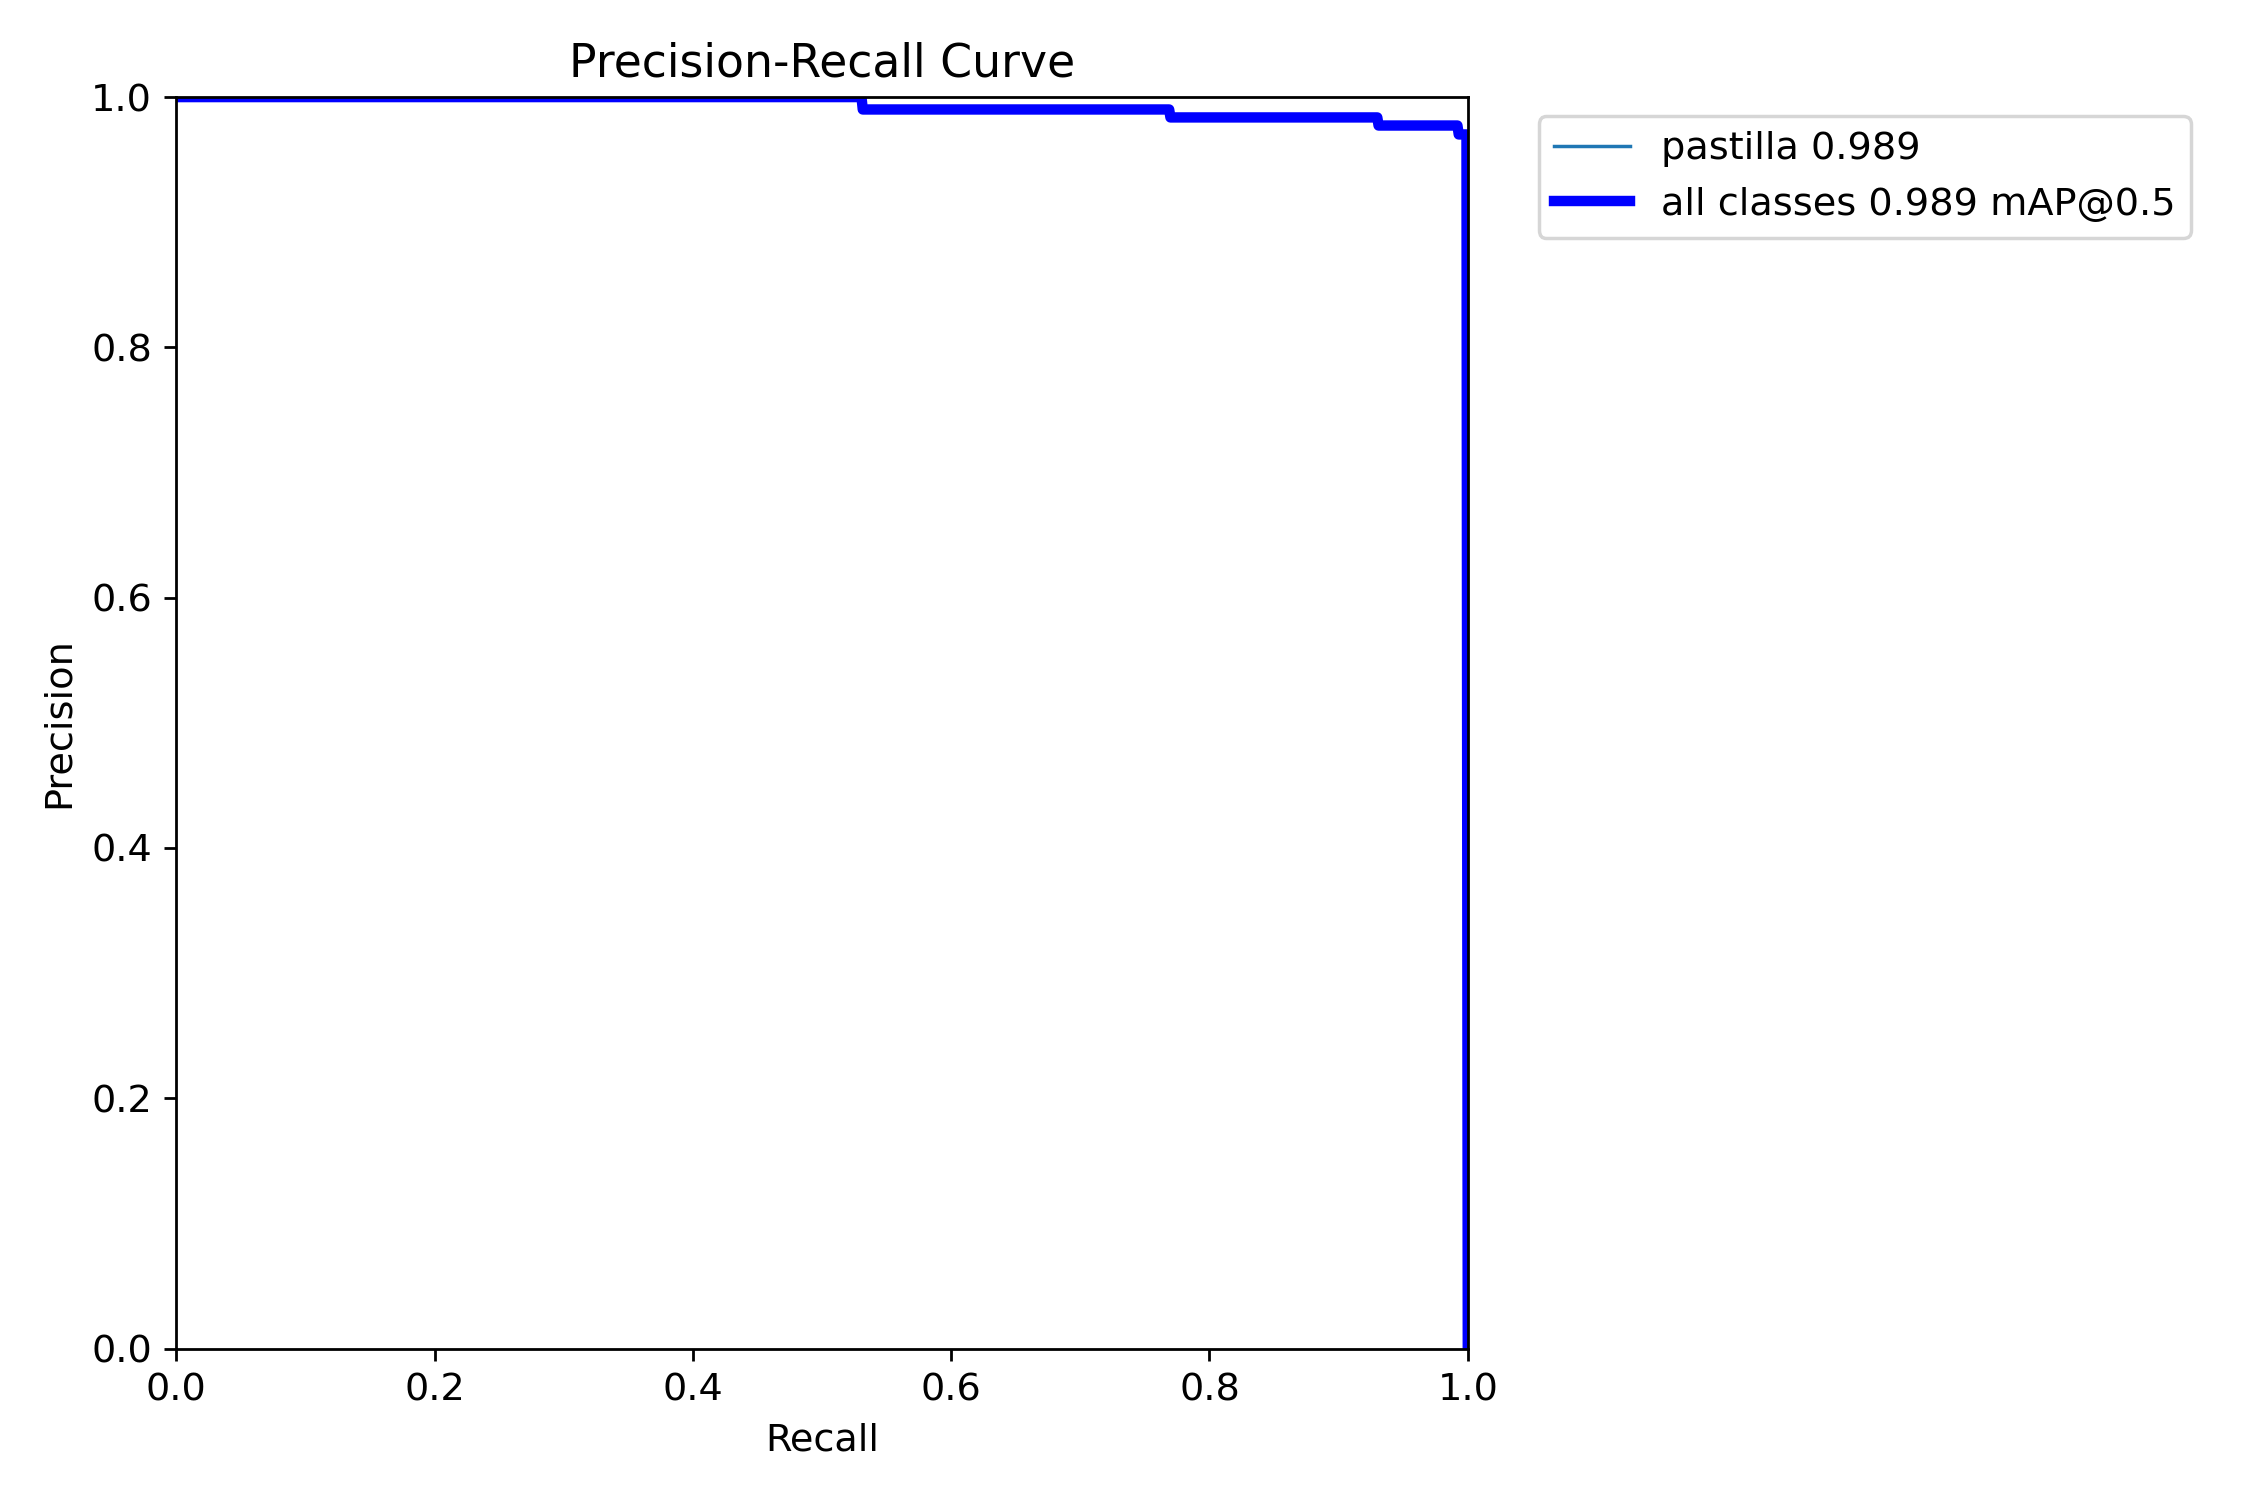
\includegraphics[width=0.82\textwidth]{imaxes/06-Procesamento automático das follas de tratamento/BoxPR_curve.png}
    \caption{Curva Precision-Recall obtida durante a validación do detector
    YOLO.}
    \label{fig:anexo-yolo-pr}
\end{figure}

\begin{figure}[htbp]
    \centering
    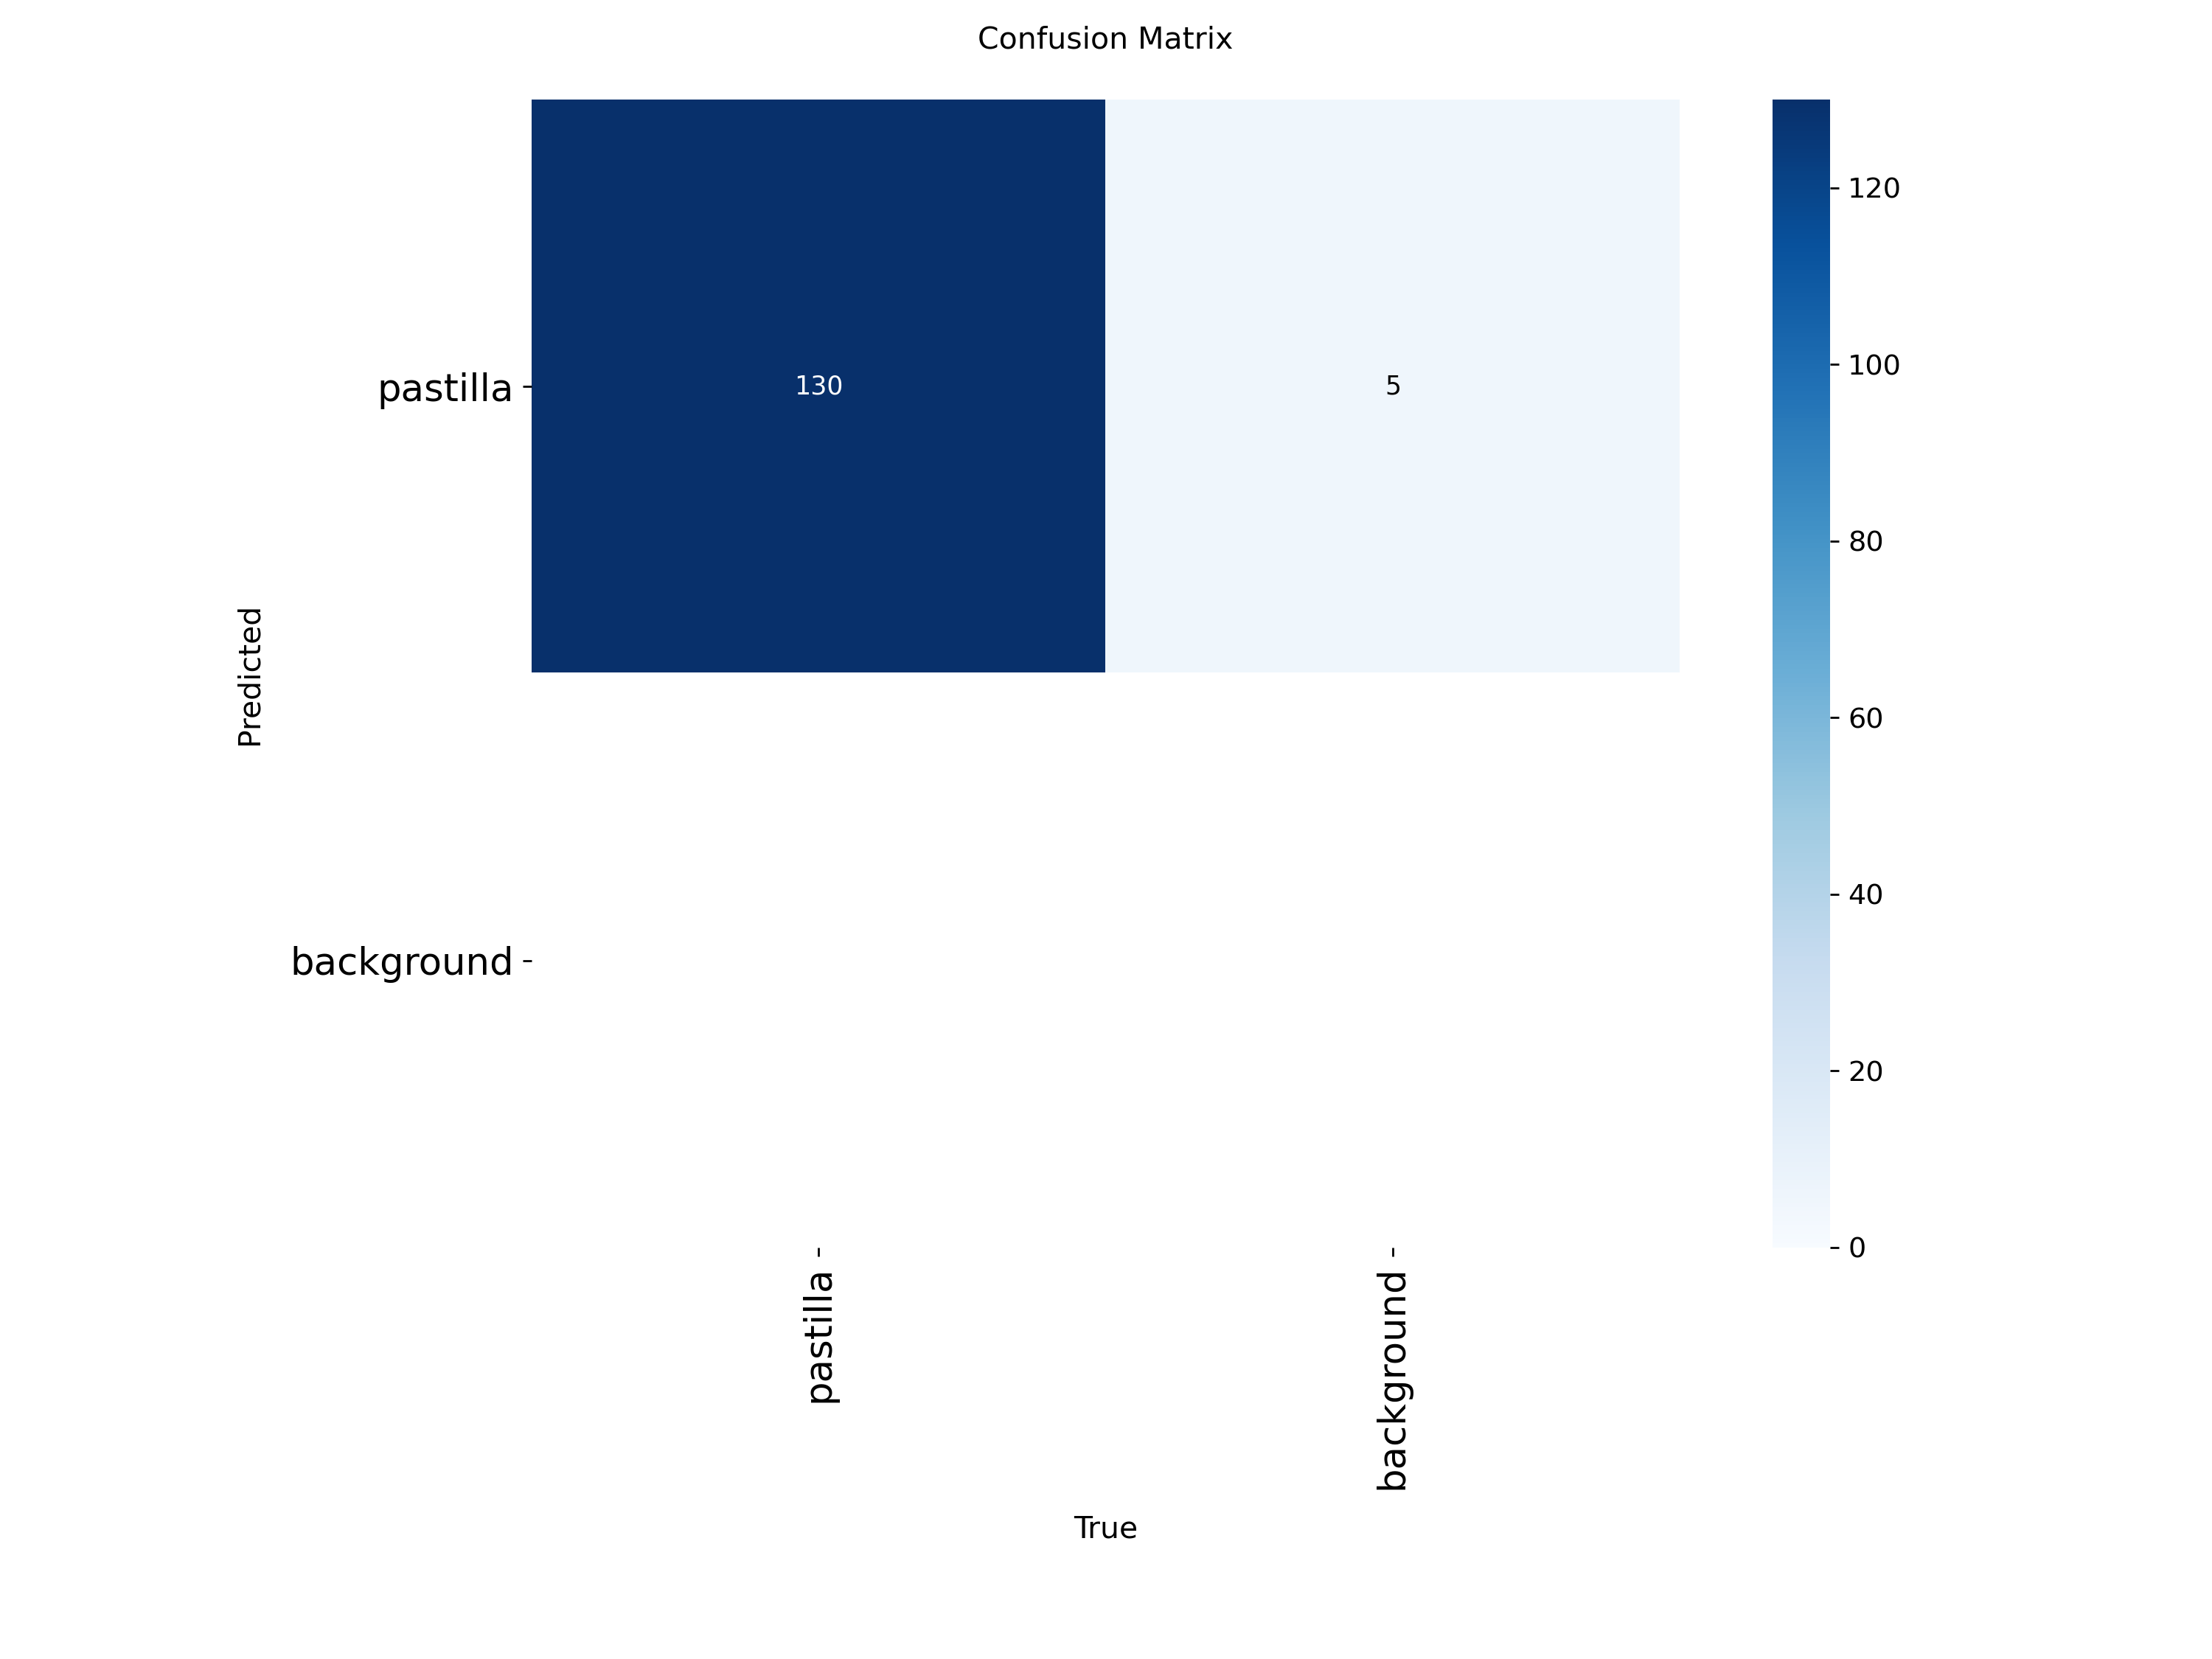
\includegraphics[width=0.82\textwidth]{imaxes/06-Procesamento automático das follas de tratamento/confusion_matrix.png}
    \caption{Matriz de confusión obtida durante a validación do detector
    YOLO.}
    \label{fig:anexo-yolo-confusion}
\end{figure}

\FloatBarrier